\documentclass{beamer}

\mode<presentation> {
	% The Beamer class comes with a number of default slide themes
	% which change the colors and layouts of slides. Below this is a list
	% of all the themes, uncomment each in turn to see what they look like.
	
	%\usetheme{default}
	%\usetheme{AnnArbor}
	%\usetheme{Antibes}
	%\usetheme{Bergen}
	%\usetheme{Berkeley}
	%\usetheme{Berlin}
	%\usetheme{Boadilla}
	%\usetheme{CambridgeUS}
	%\usetheme{Copenhagen}
	%\usetheme{Darmstadt}
	%\usetheme{Dresden}
	%\usetheme{Frankfurt}
	%\usetheme{Goettingen}
	%\usetheme{Hannover}
	%\usetheme{Ilmenau}
	%\usetheme{JuanLesPins}
	%\usetheme{Luebeck}
	\usetheme{Madrid}
	%\usetheme{Malmoe}
	%\usetheme{Marburg}
	%\usetheme{Montpellier}
	%\usetheme{PaloAlto}
	%\usetheme{Pittsburgh}
	%\usetheme{Rochester}
	%\usetheme{Singapore}
	%\usetheme{Szeged}
	%\usetheme{Warsaw}
	
	% As well as themes, the Beamer class has a number of color themes
	% for any slide theme. Uncomment each of these in turn to see how it
	% changes the colors of your current slide theme.
	
	%\usecolortheme{albatross}
	\usecolortheme{beaver}
	%\usecolortheme{beetle}
	%\usecolortheme{crane}
	%\usecolortheme{dolphin}
	%\usecolortheme{dove}
	%\usecolortheme{fly}
	%\usecolortheme{lily}
	%\usecolortheme{orchid}
	%\usecolortheme{rose}
	%\usecolortheme{seagull}
	%\usecolortheme{seahorse}
	%\usecolortheme{whale}
	%\usecolortheme{wolverine}
	
	%\setbeamertemplate{footline} % To remove the footer line in all slides uncomment this line
	%\setbeamertemplate{footline}[page number] % To replace the footer line in all slides with a simple slide count uncomment this line
	
	%\setbeamertemplate{navigation symbols}{} % To remove the navigation symbols from the bottom of all slides uncomment this line
}
\usepackage[backend=biber]{biblatex}
\setbeamertemplate{caption}[numbered]
\newcommand{\btVFill}{\vskip0pt plus 1filll}
\usepackage{algorithm}
\usepackage{amsmath}
\usepackage{caption}
\usepackage{fec}
\usepackage{xcolor}
%----------------------------------------------------------------------------------------
%	TITLE PAGE
%----------------------------------------------------------------------------------------

\title[Warm Starting Series of MILP's]{Warm Starting Series of Mixed-Integer Linear Programs}

\author{Sean Kelley} % Your name
\date{27 January 2022} % Date, can be changed to a custom date

\begin{document}
	
	\begin{frame}
		\titlepage % Print the title page as the first slide
	\end{frame}

	\begin{frame}{Overview}
		\tableofcontents
	\end{frame}

	\section{Background}
	
	\begin{frame}[t]
		\frametitle{Motivation}
		\small
		\begin{itemize}
			\item Mixed-Integer Programming has created great value in industry.
			\item One important source comes from problems solved by a series of Mixed-Integer Linear Programs (MILPs).
			\begin{itemize}
				\item Electric Grid Production Planning (Stochastic Dual Decomposition)
				\item Vehicle Routing (Branch and Price)
			\end{itemize}
			\item Many MILP instances in such series differ only by objective coefficients or bounds on their constraints.
			\item Solvers can leverage what they discover solving one MILP to more quickly solve a similar MILP (a.k.a. "Warm Start").
			\item Warm starting would enable greater performance and expand the space of tractable problems for those solved as a series of MILPs.
		\end{itemize}
		\vspace{-.25cm}
		\begin{block}{}
			This presentation details potential opportunities to warm start series of MILPs and presents problem classes whose solutions are found by solving such series.
		\end{block}
		\normalsize
	\end{frame}

	\begin{frame}[t]
		\frametitle{Simple Example}
		\footnotesize
		% what kind of information can a solver glean from a previous similar solve
		% two MILP's and their trees
		% Plug (2)'s bounds into (1)'s subproblems (get the right)
		% Gives us a branching decision (disjunction), primal solutions and dual bounds
		% Get similar tree by plugging in new objective instead of bounds
		\begin{columns}[T]
			\begin{column}{0.45\textwidth}
				\vspace{-.75cm}
				\begin{align}
					\begin{split}
						\text{max} \{ &x + 4y : -\frac{x}{2} + y \leq 2, \\
						&x + \frac{y}{2} \leq 4, (x, y) \in \Zmbb^2_+ \} 
					\end{split}
					\label{left}
				\end{align}
				\vspace{-.5cm}
				\begin{figure}[h]
					\resizebox{.45\textwidth}{!}{%
						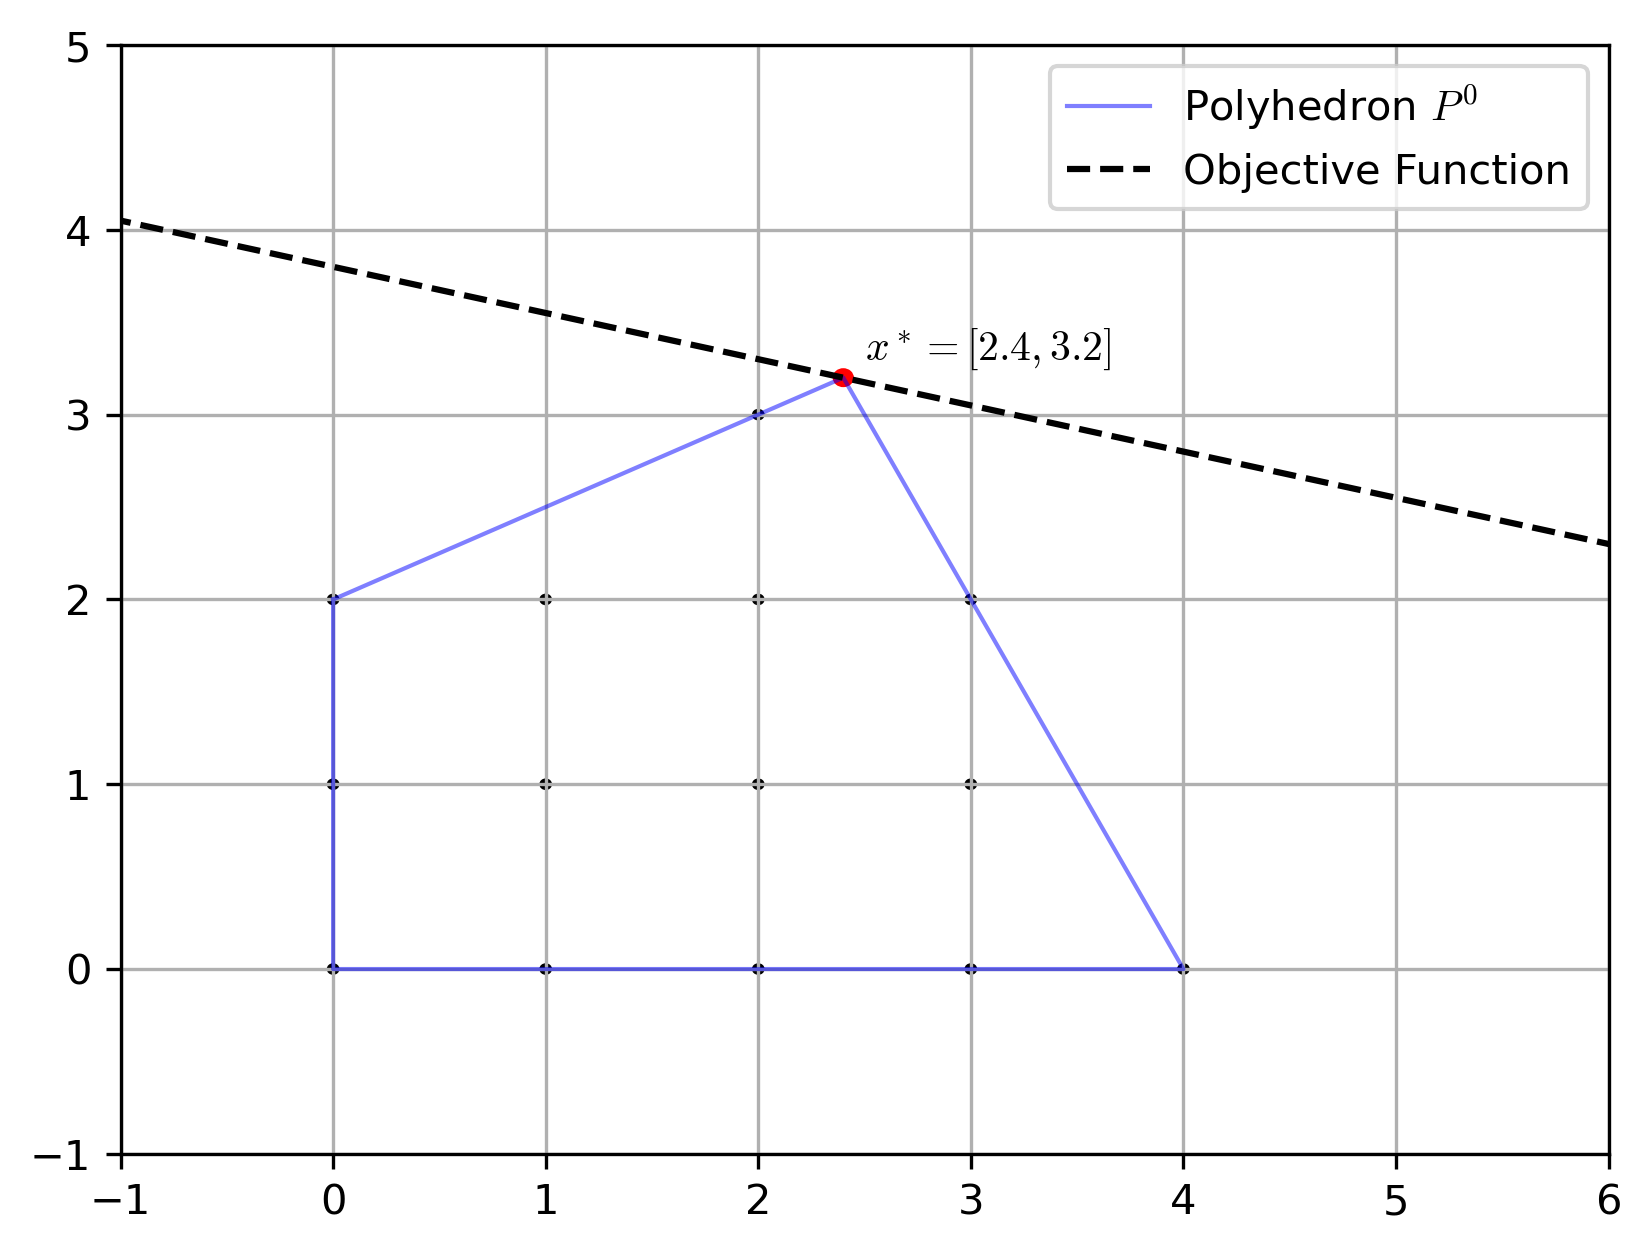
\includegraphics[]{P0.png}
					}
					% \caption{Node 0 LP relaxation}
					\label{p:root}
				\end{figure}
				\centering
				Branch on $ x \leq 2 $ or $ x \geq 3 $
				\begin{figure}[]
					\centering
					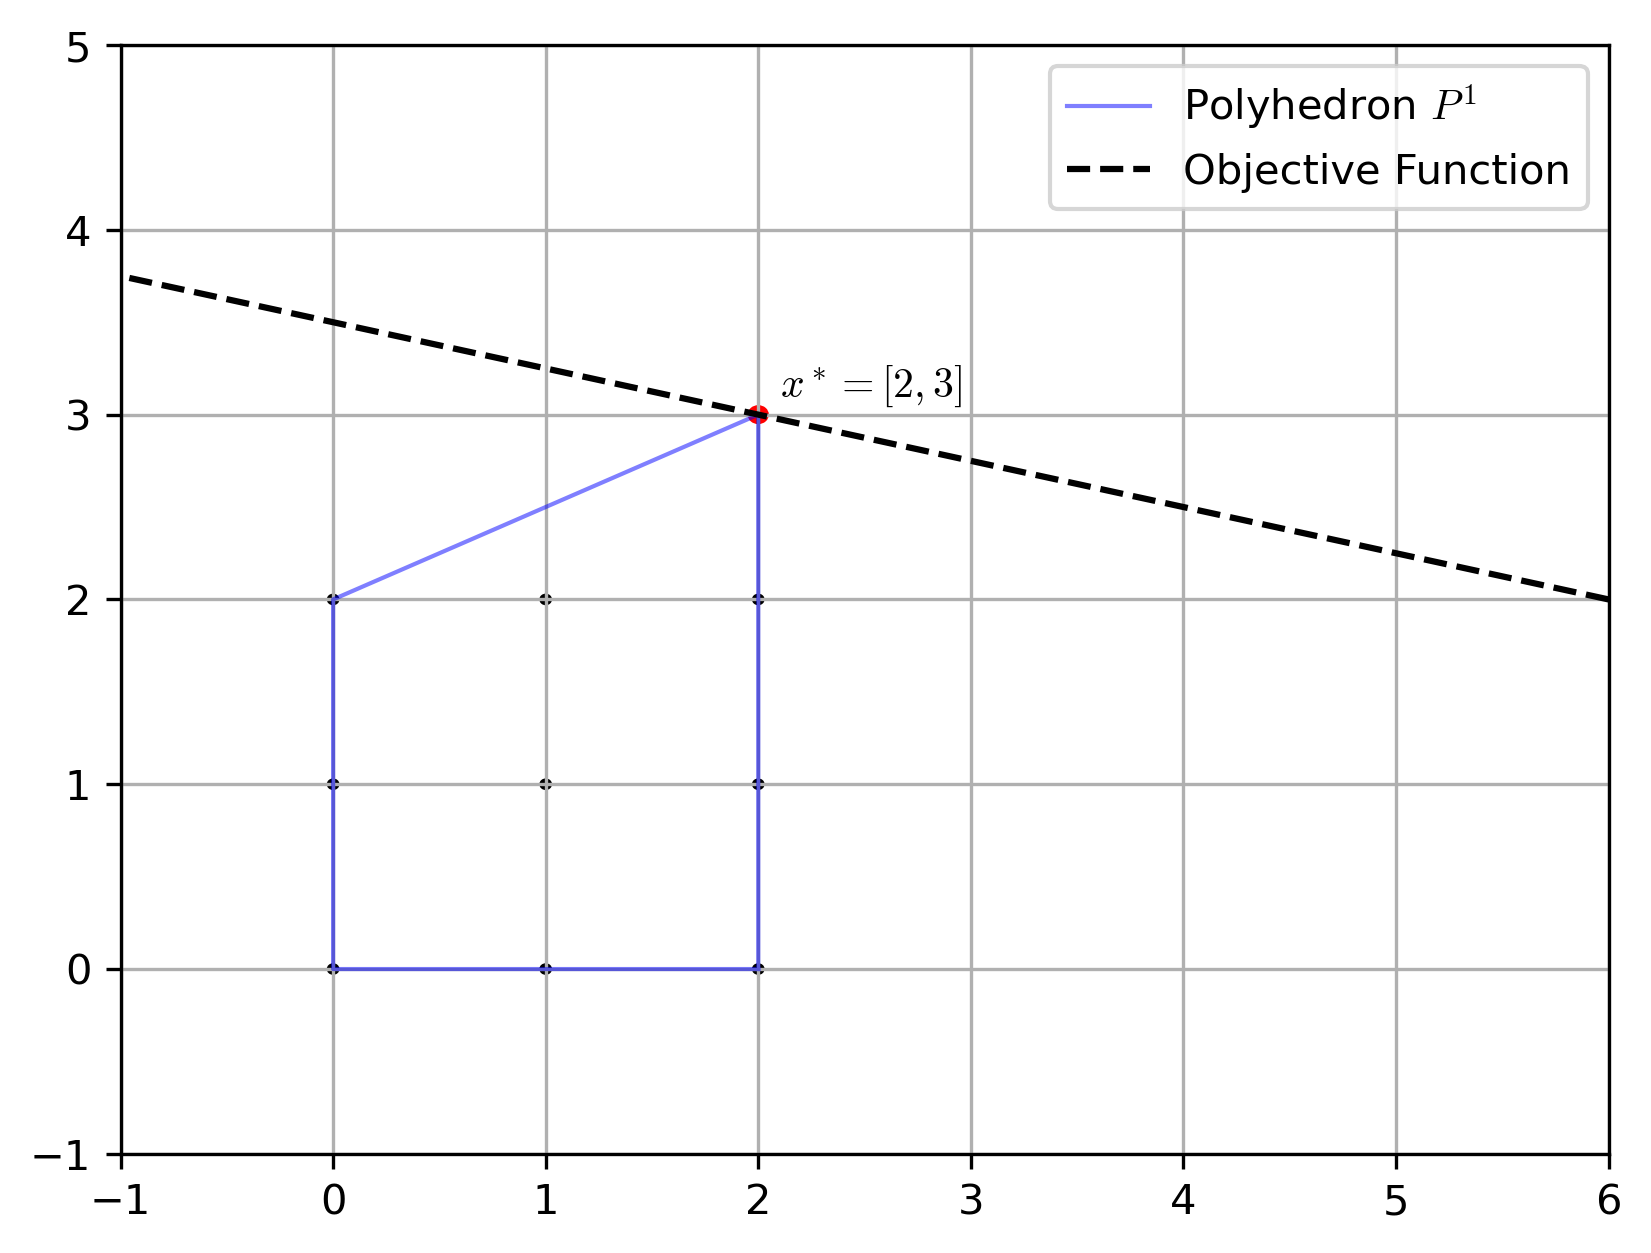
\includegraphics[width=.45\textwidth]{P1.png}
					\hfill
					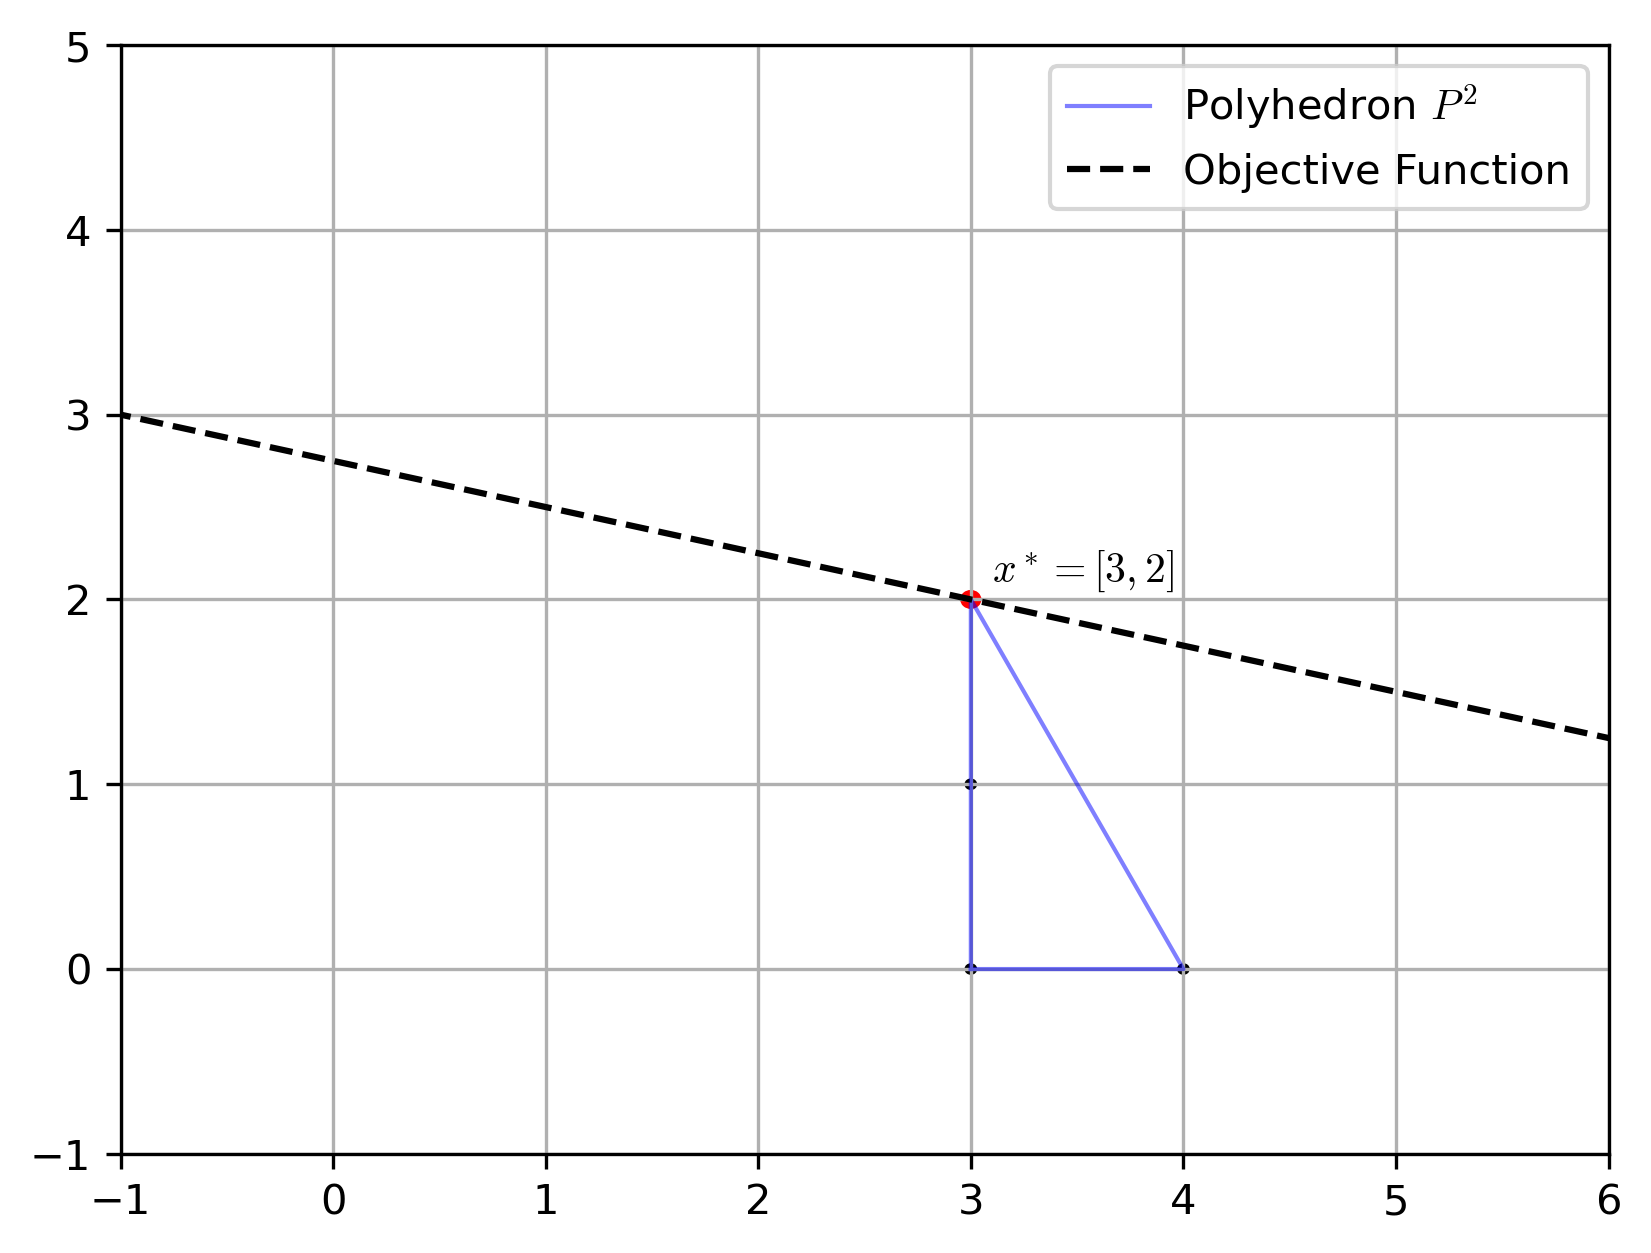
\includegraphics[width=.45\textwidth]{P2.png}
					\captionsetup{font=footnotesize,labelfont=footnotesize}
					\caption{(\ref{left})'s Branch and Bound tree}
					\label{p:before}
				\end{figure}
			\end{column}
			\begin{column}{0.10\textwidth}
				\vspace{2.5cm}
				\centering
				Update bounds $ \implies $
			\end{column}
			\begin{column}{0.45\textwidth}
				\vspace{-.75cm}
				\begin{align}
					\begin{split}
						\text{max} \{ &x + 4y : -\frac{x}{2} + y \leq 3, \\
						&x + \frac{y}{2} \leq 5, (x, y) \in \Zmbb^2_+ \} 
					\end{split}
					\label{right}
				\end{align}
				\vspace{-.5cm}
				\begin{figure}[h]
					\resizebox{.45\textwidth}{!}{%
						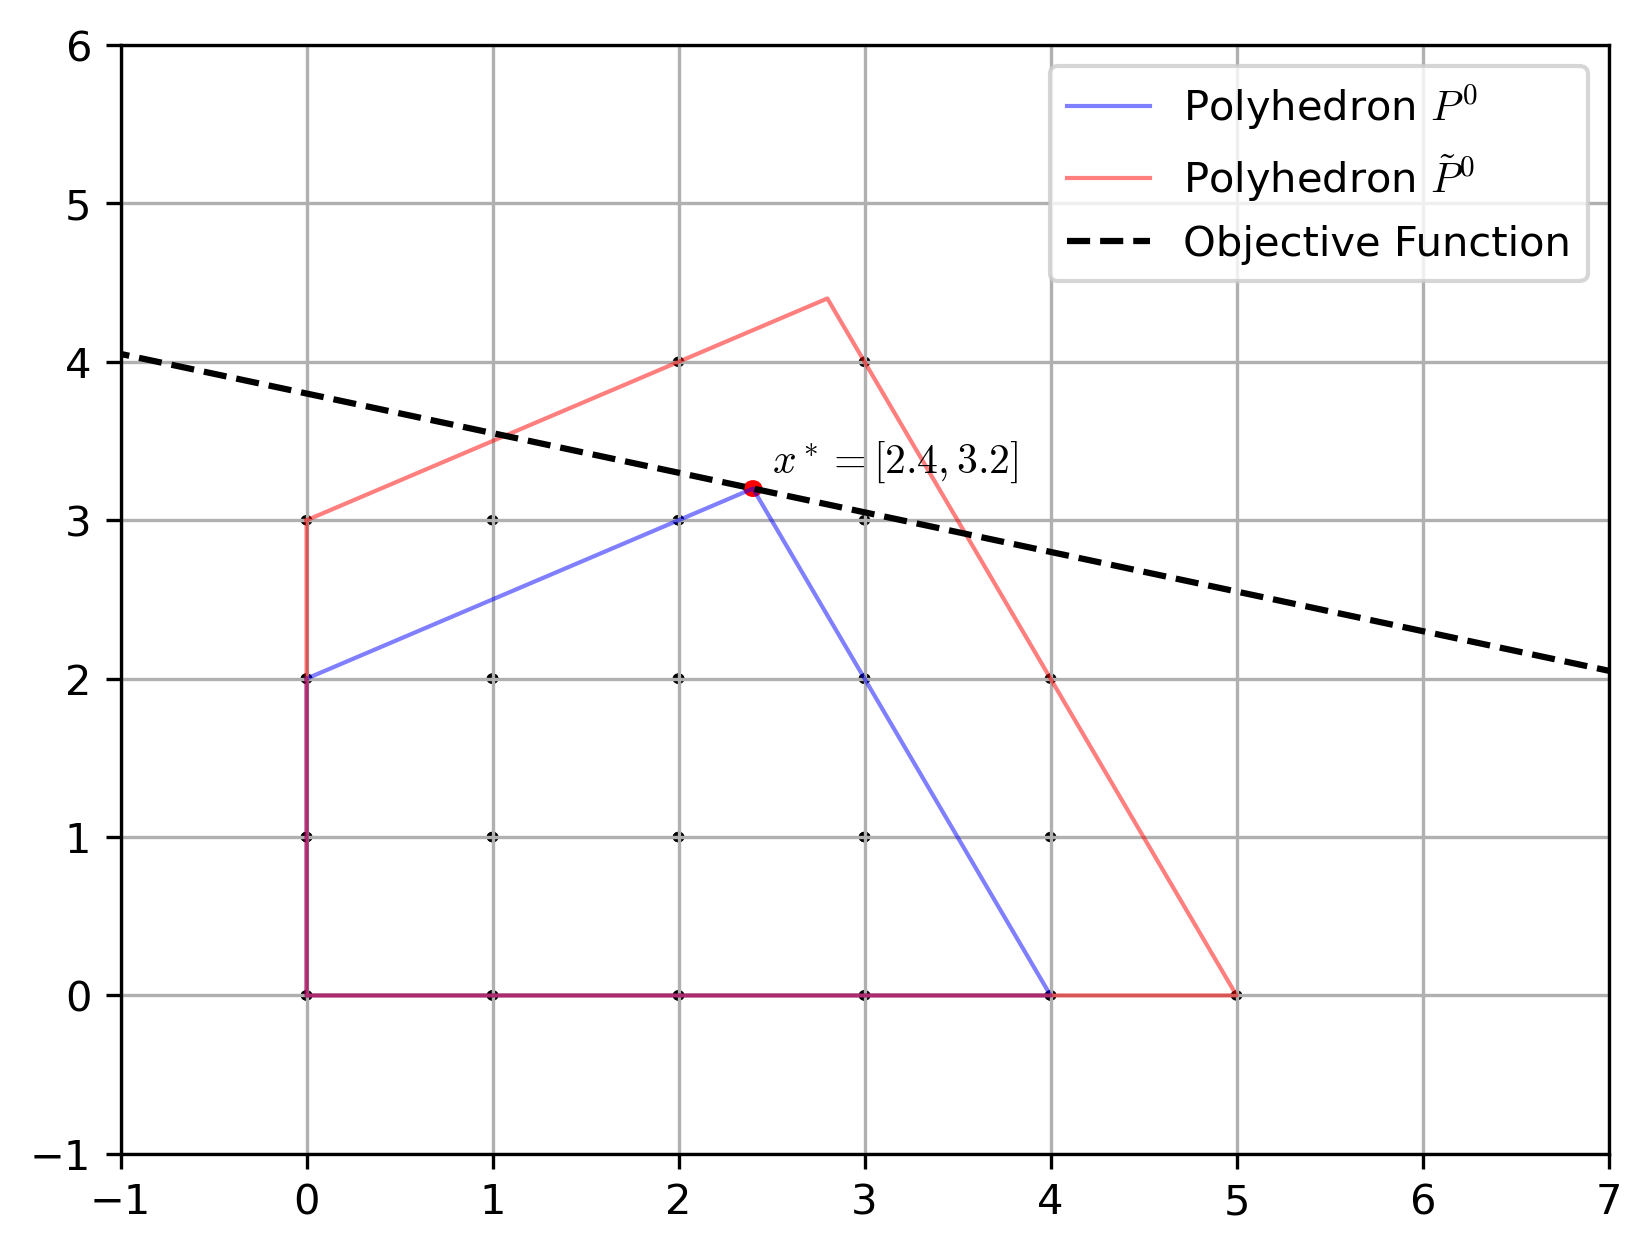
\includegraphics[]{P0_prime.png}
					}
					% \caption{Node 0 LP relaxation}
					\label{p:root_prime}
				\end{figure}
				\centering
				Branch on $ x \leq 2 $ or $ x \geq 3 $
				\begin{figure}[]
					\centering
					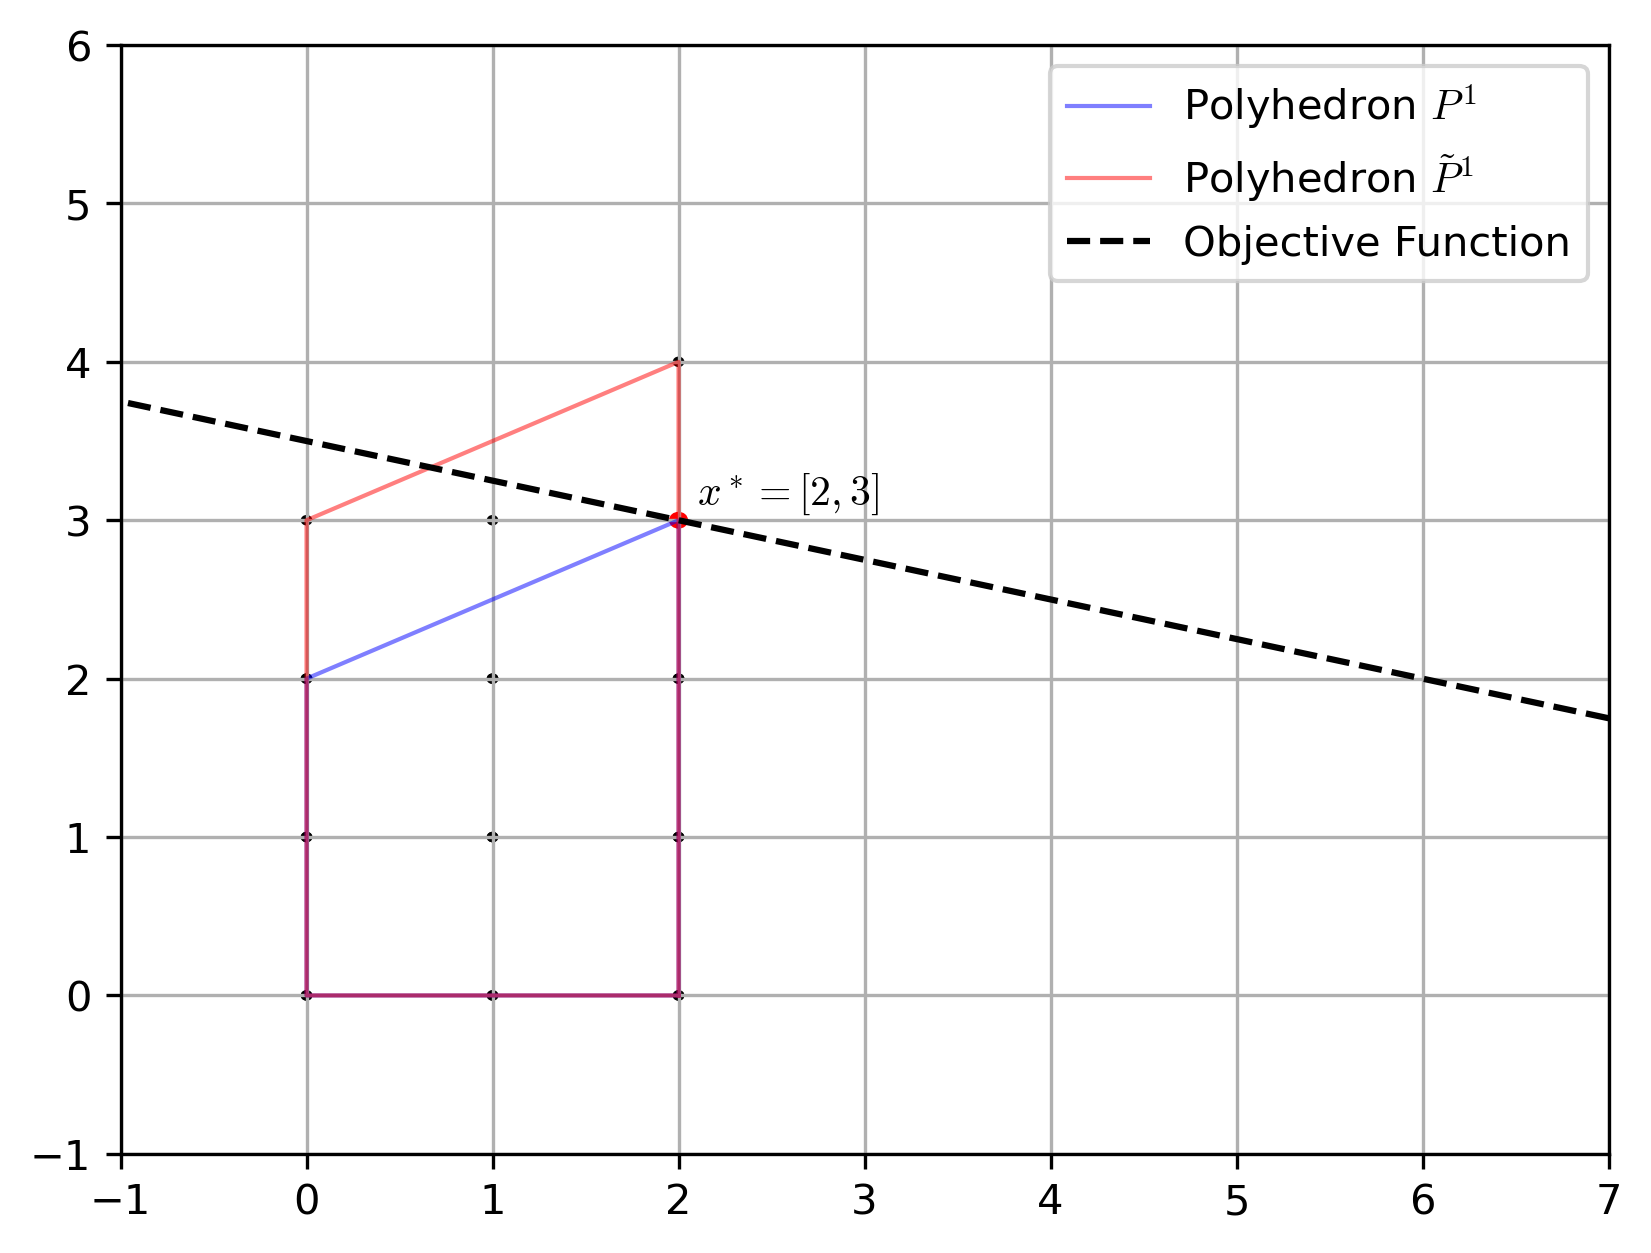
\includegraphics[width=.45\textwidth]{P1_prime.png}
					\hfill
					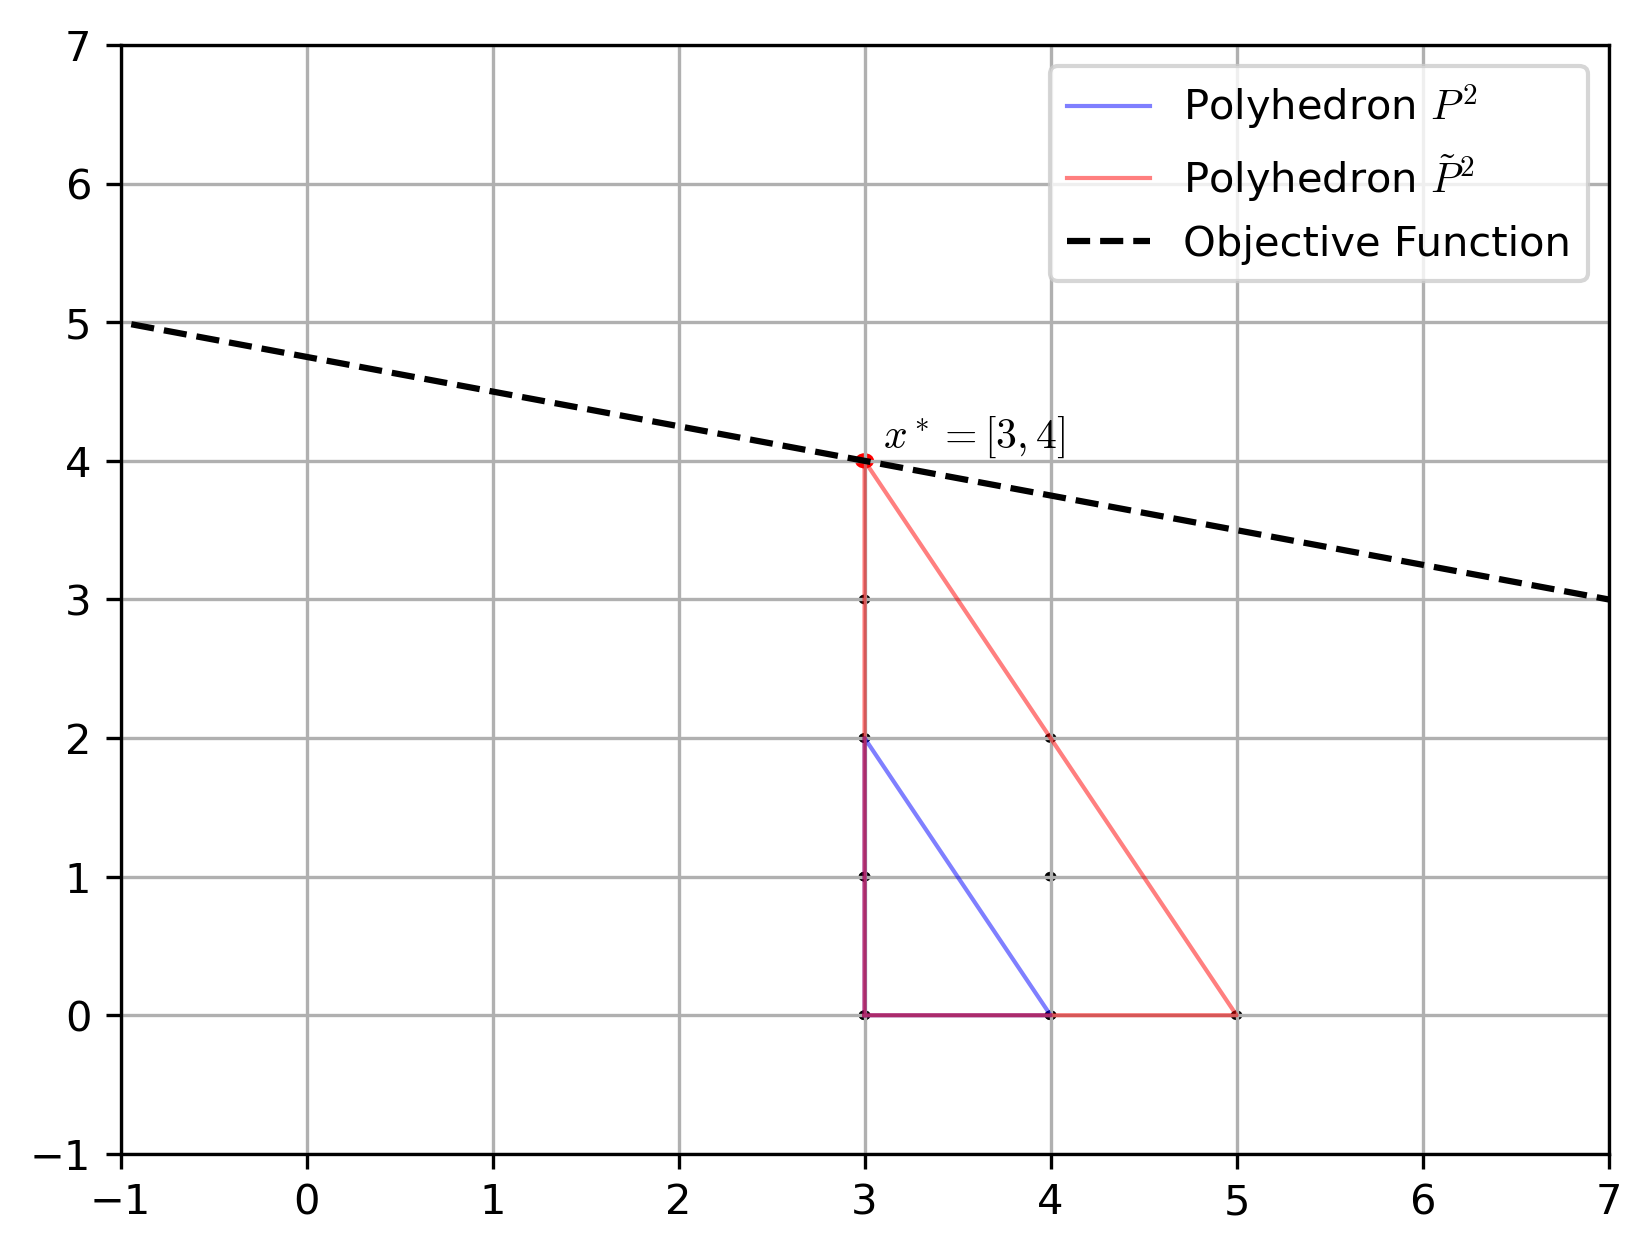
\includegraphics[width=.45\textwidth]{P2_prime.png}
					\captionsetup{font=footnotesize,labelfont=footnotesize}
					\caption{(\ref{right})'s Branch and Bound tree}
					\label{p:after}
				\end{figure}
			\end{column}
		\end{columns}
		\vspace{-.25cm}
		\begin{block}{}
			After solving (\ref{left}), we can get a tree for (\ref{right}) without another solve by substituting (\ref{right})'s bounds in each subproblem of (\ref{left}).
		\end{block}
		\normalsize
	\end{frame}

	\begin{frame}[t]
		\frametitle{Three Ways to Warm Start}
		\small
		\vspace{-.25cm}
		% how can we use this information to help speed up our solver?
		\begin{block}{}
			After updating the objective and constraint bounds in all subproblems of Branch and Cut, we have the following three approaches to warm start.
		\end{block}
		\begin{itemize}
			\item [(a)] Good warm start:
			\begin{itemize}
				% if we relaxed our constraints or changed objective
				\item Recalculate the primal bound.
				\item Restart Branch and Cut from the root node.
				% super simple to do
			\end{itemize}
			\item [(b)] Better warm start:
			\begin{itemize}
				% Can recycle cuts by ensuring their validity
				\item Parameterize cuts.
				\item Recalculate the primal and/or dual bounds.
				\item Restart Branch and Cut from the leaf nodes.
				% works even when constraint bounds tighten, yields better primal/dual bounds, saves us from resolving same subproblems
			\end{itemize}
			\item [(c)] Hypothesized best warm start:
			\begin{itemize}
				\item Parameterize cuts.
				\item Add to the root relaxation cuts valid for all terminal subproblems.
				\item Restart Branch and Cut from the root node.
				% what do these cuts look like?
				% why would we want to toss out so many solved subproblems?
			\end{itemize}
		\end{itemize}
		\normalsize
	\end{frame}

	\begin{frame}[t]
		\frametitle{Valid Cuts for All Terminal Subproblems}
		\small
		\begin{columns}[T]
			% a cut valid for the subproblems of the second instance
			\begin{column}{0.4\textwidth}
				\vspace{-.25cm}
				\begin{figure}[h]
					\resizebox{\textwidth}{!}{%
						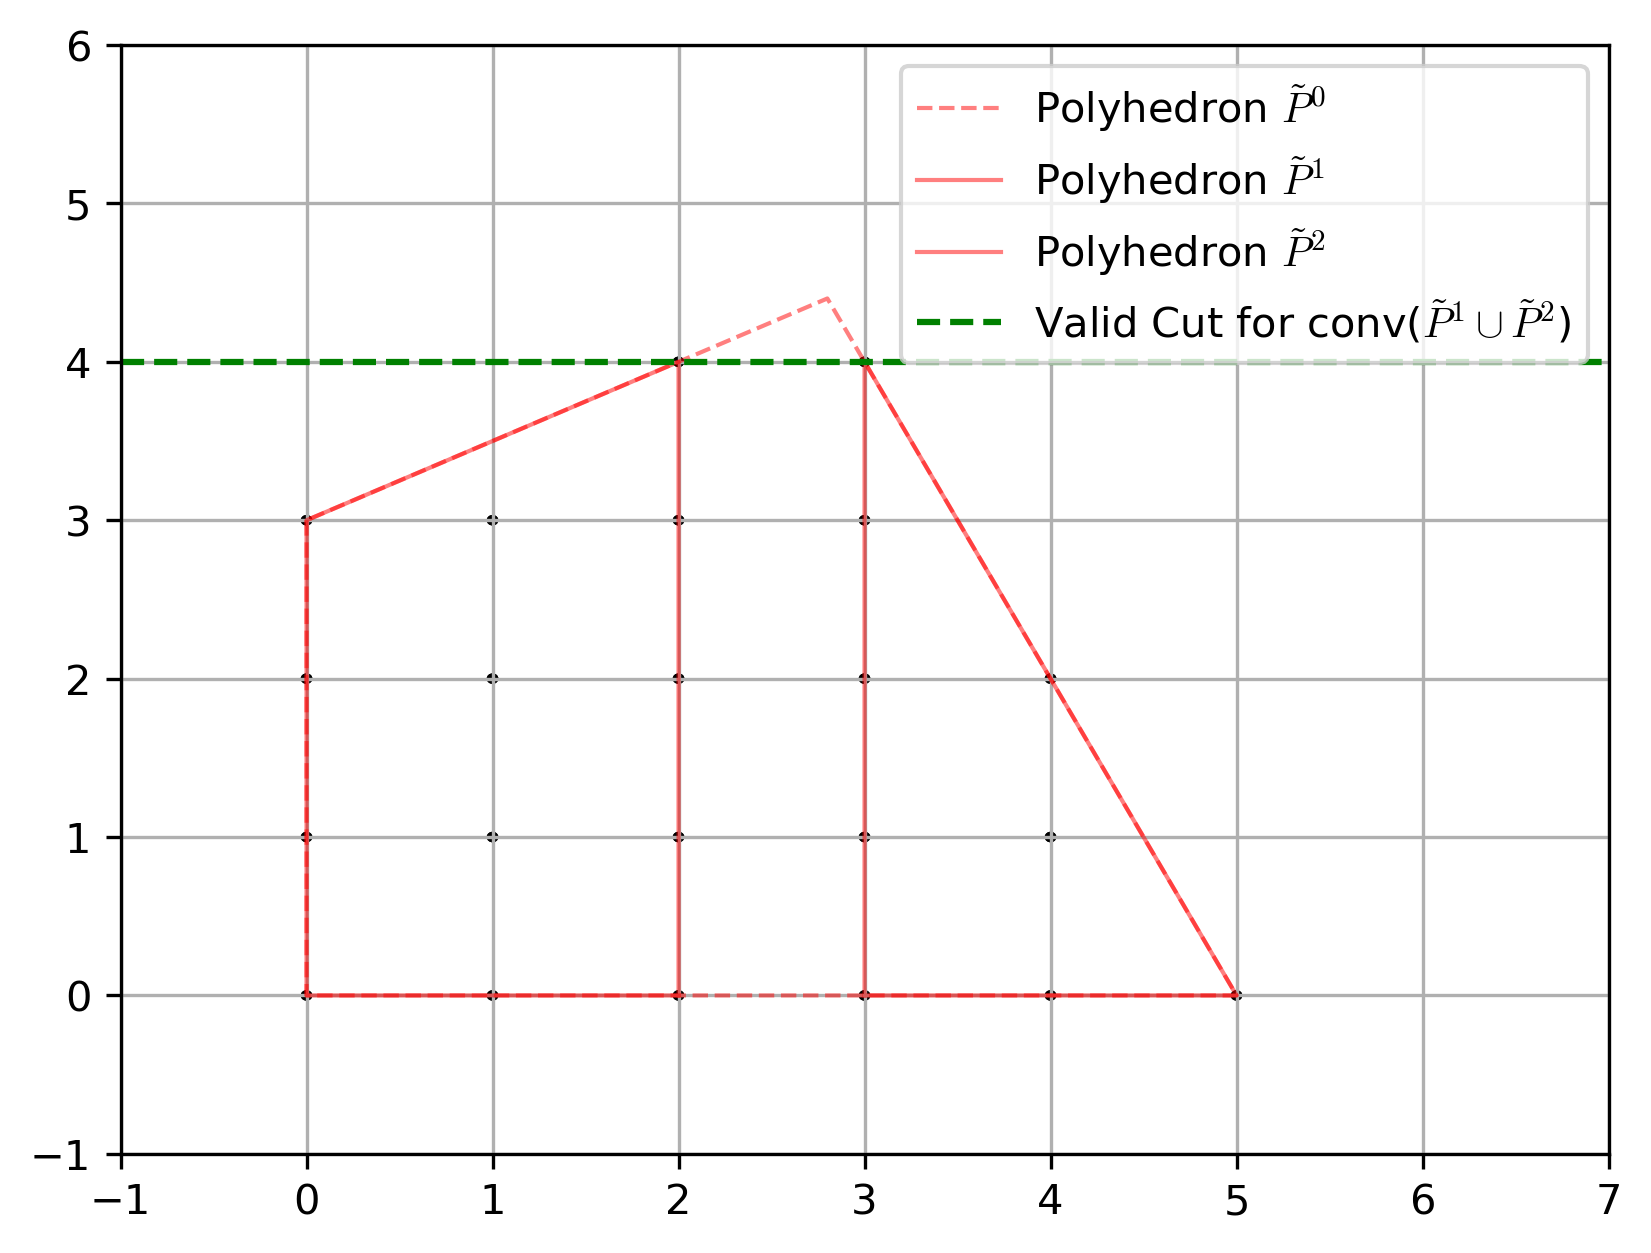
\includegraphics[]{PD_prime.png}
					}
					\caption{A cut valid for both of (\ref{right})'s subproblems}
					\label{p:hull}
				\end{figure}
			\end{column}
			\begin{column}{0.6\textwidth}
				\begin{itemize}
					\item We are motivated to explore (c) because:
					\begin{itemize}
						\item It maintains (b)'s tightened relaxation while removing need to explore all subproblems.
						\item It can remain effective when objective or constraint bounds change greatly.
						% bc where we add cuts depends on the new objective or bounds
					\end{itemize}
					\item We want to find cuts such that:
					\begin{itemize}
						\item No terminal subproblem is violated.
						\item Some estimate of the solution is maximally violated.
					\end{itemize}
				\end{itemize}
			\end{column}
		\end{columns}
		\vspace{.5cm}
		\begin{block}{}
			We can find cuts valid for all terminal subproblems by formulating and solving a LP known as the Cut Generating LP (CGLP).
		\end{block}
		\normalsize
	\end{frame}

	\begin{frame}[t]
		\frametitle{Updating a Branch and Bound Tree for Warm Starting}
		\small
		% before going into how we find these cuts, we need to define how we update the tree off which we base them.
		\begin{itemize}
			\item Let $ t $ be the index of a node in a Branch and Bound tree.
			\item Define the feasible region of the LP subproblem in node $ t $ as
			\begin{align*}
				P^{t} =& \{x \in \Rmbb^n : A^{t} x \geq b^{t}, u^{t} \geq x \geq l^{t} \}
			\end{align*}
			where
			\begin{itemize}
				\item $ A^{t} = \begin{bmatrix} A \\ \Pi^{t} \end{bmatrix}$ and $ b^{t} = \begin{bmatrix} b \\ \Pi_0^{t}(b) \end{bmatrix} $.
				\item $ b $ is the constraint bounds for the warm started MILP.
				\item ($ \Pi^{t}, \Pi_0^{t}(b) $) represent parameterized valid inequalities derived from cut generation routines of node $ t $ and its ancestors in the previous solve.
				\item $ u^{t} $ and $ l^{t} $ are bounds on $ x $ from branching in the previous solve.
			\end{itemize}
			\item Let $ \mathcal{T} $ be the terminal nodes of a Branch and Bound tree.
			\item Cuts valid for all terminal subproblems are equivalent to those valid for
			\begin{align*}
				P_D = \text{conv}(\underset{t \in \mathcal{T}}{\bigcup} P^{t})
			\end{align*}
		\end{itemize}
		\normalsize
	\end{frame}

	\begin{frame}[t]
		\frametitle{Deriving the Cut Generating LP}
		\small
		% with our tree defined, lets now define sufficient cuts
		\begin{itemize}
			% first two bullets just say a linear combo of constraints is itself a valid inequality
			\item Let $ \mu^{t} \in \Rmbb_+^m $, $ w^{t} \in \Rmbb_+^n $, $ v^{t} \in \Rmbb_+^n $, and $ I_n $ be the $ n $-dimensional identity matrix. 
			\item The following is a valid inequality for $ P^{t} $:
			\begin{align}
				{A^{t}}^T \mu^{t} + I_n w^{t} - I_n v^{t} \geq {b^{t}}^T \mu^{t} + {l^{t}}^T w^{t} - {u^{t}}^T v^{t} \label{e:valid_inequality}
			\end{align}
			% third bullet says to find an inequality valid for each of the linear combos 
			\item Let $ \pi \in \Rmbb^n $ and $ \pi_0 \in \Rmbb $ satisfy the following:
			\begin{align}
				\begin{split}
					\pi &\geq {A^{t}}^T \mu^{t} + I_n w^{t} - I_n v^{t} \\
					\pi_0 & \leq {b^{t}}^T \mu^{t} + {l^{t}}^T w^{t} - {u^{t}}^T v^{t}
				\end{split} \; \text{ for all } t \in \mathcal{T} \label{e:disjunctive_inequality}
			\end{align}
			% thus its valid for all terminal nodes of the MILP
			\item Since (\ref{e:valid_inequality}) is a valid inequality for each LP in $ \mathcal{T} $, it follows $ \pi^T x \geq \pi_0 $ is a valid inequality for all $ x \in P_D $.
		\end{itemize}
		\normalsize
	\end{frame}

	\begin{frame}[t]
		\frametitle{Deriving the Cut Generating LP}
		\small
		\vspace{-.25cm}
		\begin{itemize}
			% now that we know what makes a cut feasible, we can find the one that cuts off the estimate as much as possible
			\begin{block}{}
				We can generate a cut valid for all terminal subproblems that maximally violates a solution estimate by solving the CGLP.
			\end{block}
			\item Let $ \bar{x} \in \Rmbb^n $ be an estimate of the optimal solution the MILP instance.
			\item We define (CGLP) as follows:
			\begin{equation} \tag{CGLP}
				\begin{alignedat}{2} \label{e:cglp} 
					\text{minimize } \; \; \qquad & \pi^T \bar{x} - \pi_0 && \\
					\text{subject to } \qquad \pi & \geq {A^{t}}^T \mu^{t} + I_n w^{t} - I_n v^{t} && \;  t \in \mathcal{T} \\
					\pi_0 & \leq {b^{t}}^T \mu^{t} + {l^{t}}^T w^{t} - {u^{t}}^T v^{t} && \; t \in \mathcal{T} \\
					1 & = \sum_{t \in \mathcal{T}} \big( \sum_{j=1}^{m^t} \mu_j^{t} + \sum_{i=1}^{n} w_i^{t} + \sum_{i=1}^{n} v_i^{t} \big) && \\
					& \mu^{t} \in \Rmbb_+^{m^t}, \; w^{t} \in \Rmbb_+^n \; v^{t} \in \Rmbb_+^n && t \in \mathcal{T}
				\end{alignedat}
			\end{equation}
			\vspace{-.25cm}
			\begin{block}{}
				Warm start method (c) is completed by adding the solutions to (CGLP) as cuts to the root relaxation.
			\end{block}
		\end{itemize}
		\normalsize
	\end{frame}

	\section{Applications}
	
	\begin{frame}[t]
		\frametitle{Restarting MILP's}
		\small
		\vspace{0cm}
		% thus concludes methodology, so let's talk applications
		\begin{itemize}
			\item Warm starting with a tightened root LP relaxation can be preferred to a partial tree already found on a looser root relaxation.
			\item We aim to identify problem classes where there is a strong preference for the former.
			\item When this is true, a partial solve followed by warm start method (c) takes less time than solving the instance cold.
			\item The idea then is as follows:
			\begin{itemize}
				\item Solve LP relaxations for certain number of nodes.
				\item Generate CGLP cuts against this tree.
				\item Tighten root node with these cuts.
				\item Restart Branch and Cut from beginning with tightened root relaxation.
			\end{itemize}
		\end{itemize}
		\vspace{0cm}
		\begin{block}{}
			If many problem classes exist where the above is beneficial, this would dramatically change how solvers work today.
		\end{block}
		\normalsize
	\end{frame}
	
	\begin{frame}[t]
		\frametitle{Dual Decomposition for Stochastic MILP}
		\small
		\vspace{-.25cm}
		% for a more practical example, we're also looking at warm starting decomposable MILP's like
		\begin{itemize}
			\item Let $ S^j := \{(x, y^j): Ax \leq b, x \in X, T^j x + w y^j \leq h^j, y^j \in Y\} $
			\item A multistage stochastic MILP can be formulated as follows:
			% the deterministic formulation
			\begin{align}
				\text{max} \left\{ c^T x + \sum_{j=1}^{r} p^j {q^j}^T y^j : (x, y^j) \in S^j \text{ for } j \in [r] \right\} \label{smilp1}
			\end{align}
			\item It can be reformulated as follows:
			% make scenarios independent but tie them together with linking constraints
			\begin{align}
				\text{max} \left\{ \sum_{j=1}^{r} p^j (c^T x^j + {q^j}^T y^j) : (x^j, y^j) \in S^j \text{ for } j \in [r], x^1 = ... = x^r \right\} \label{smilp2}
			\end{align}
			\item For $ H^j $ such that $ \sum_{j=1}^{r} H^j x^j = 0 $ is equivalent to $ x_1 = ... = x_r $, (\ref{smilp1}) and (\ref{smilp2}) can have an upper bound decomposed as follows:
			% for sufficiently structured H, we can minimize its product with x, remove it from the constraints, and get the following upper bound
			\begin{align}
				& \qquad \qquad \qquad \qquad \qquad \underset{\lambda}{\text{ min }} D(\lambda) \label{LD} \tag{LD} \\
				D(\lambda) &= \text{max} \left\{ \sum_{j=1}^{r} p^j (c^T x^j + {q^j}^T y^j) + \lambda(H^j x^j) : (x^j, y^j) \in S^j \text{ for } j \in [r] \right\} \nonumber
			\end{align}
		\end{itemize}
		\normalsize
	\end{frame}
	
	\begin{frame}[t]
		\frametitle{Dual Decomposition for Stochastic MILP}
		\small
		\vspace{0cm}
		% when we look at how we solve (LD), we see a lot of opportunity to warm start
		\begin{itemize}
			% the solve method is
			\item $ D(\lambda) $ consists of $ r $ independent MILP's.
			\item (LD) is solved by a subgradient algorithm. We branch on the average value of $ x $ in (LD)'s solution and bound (LD) again until $ x^j $ are all identical.
			% the opportunities for warm starting are
			\item Notice there are $ r $ series of MILPs sharing similar structure:
			\begin{itemize}
				\item MILP $ j $ in $ D(\lambda) $ differs from MILP $ j $ in $ D(\lambda') $ only by objective.
				\item MILP $ j $ in $ D(\lambda) $ before branching differs from MILP $ j $ in $ D(\lambda) $ after branching only by variable bounds.
			\end{itemize}
		\end{itemize}
		\vspace{1.5cm}
		\begin{block}{}
			Since solving a multistage Stochastic MILP involves solving multiple series of potentially difficult MILPs, the warm starting techniques presented earlier could be beneficial to the solution method.
		\end{block}
		\normalsize
	\end{frame}
	
	\section{Closing Thoughts}
	
	\begin{frame}[t]
		\frametitle{Warm Starting Big Picture}
		\small
		\begin{block}{}
			We have a couple approaches at our disposal for warm starting a MILP from a previously solved one.
		\end{block}
		\begin{itemize}
			\item [(a)] Good warm start:
			\begin{itemize}
				\item Recalculate the primal bound.
				\item Restart Branch and Cut from the root node.
			\end{itemize}
			\item [(b)] Better warm start:
			\begin{itemize}
				\item Parameterize cuts.
				\item Recalculate the primal and/or dual bounds.
				\item Restart Branch and Cut from the leaf nodes.
			\end{itemize}
			\item [(c)] Hypothesized best warm start:
			\begin{itemize}
				\item Parameterize cuts.
				\item Add to the root relaxation cuts valid for all terminal subproblems.
				\item Restart Branch and Cut from the root node.
			\end{itemize}
		\end{itemize}
		\normalsize
	\end{frame}
	
	\begin{frame}[t]
		\frametitle{Next Steps}
		\small
		\begin{columns}[T]
			\begin{column}{0.45\textwidth}
				There are a few other problem classes we look to test the effectiveness of warm starts:
				\begin{itemize}
					\item Multiobjective MILP
					\item Primal Heuristics (RINS)
					\item Bilevel MILP
					\item Real-Time MILP
					\item MINLP
				\end{itemize}
			\end{column}
			\begin{column}{0.45\textwidth}
				We have the following next tasks in mind:
				\begin{itemize}
					\item Make cut generation numerically safe.
					\item Parametrize cut generation.
					\item Implement algorithms for each problem class.
					\item Run experiments for each algorithm comparing warm started version to current algorithms.
				\end{itemize}
			\end{column}
		\end{columns}
		\begin{block}{}
			We intend to test our warm starting methods against the problem classes mentioned in this presention to determine which can leverage these approaches to more effeciently be solved.
		\end{block}
		\normalsize
	\end{frame}

	\section{Index}

	\begin{frame}[t]
		\frametitle{Simple Approach to Warm Starting}
		\small
		\begin{itemize}
			\item Warm starting means to reuse a Branch and Bound tree from solving a previous MILP when solving a new one.
			\item One approach is to reevaluate leaf nodes' solutions at the new MILP’s objective and RHS to set applicable bounds. Then leaf nodes are placed into a priority queue, and Branch and Cut resumes.
			\item This approach has the following advantages:
			\begin{itemize}
				\item [(a)] When only the objective changes, all previously feasible solutions remain feasible. We can start the primal bound as the one with the best evaluation of the new objective.
				\item [(b)] When only the RHS changes, each node's dual LP relaxation maintains the same feasible region. We can start the dual bound of each node as its previous dual LP solution evaluated at the new RHS.
				\item [(c)] Restarting from the leaf nodes prevents us from having to branch and bound to regenerate them in the new instance.
			\end{itemize}
		\end{itemize}
		\normalsize
	\end{frame}

	\begin{frame}[t]
		\frametitle{Simple Approach to Warm Starting}
		\small
		\begin{itemize}
			\item Warm starting means to reuse a Branch and Bound tree from solving a previous MILP when solving a new one.
			\item One approach is to reevaluate leaf nodes' solutions at the new MILP’s objective and RHS to set applicable bounds. Then leaf nodes are placed into a priority queue, and Branch and Cut resumes.
			\item This approach has the following disadvantages:
			\begin{itemize}
				\item [(a)] The primal or dual bound is weak if the objective or RHS changes significantly.
				\item [(b)] Potentially many leaf nodes will need to be branched.
				\item [(c)] Generated cuts may no longer be valid if RHS changed.
			\end{itemize}
		\end{itemize}
		\vspace{.5cm}
		\begin{block}{}
			Starting a MILP solve with a Branch and Bound tree from a previous solve can be a simple and quick way to improve performance, but such an approach is not a panacea.
		\end{block}
		\normalsize
	\end{frame}

	\begin{frame}[t]
		\frametitle{Motivating the Cut Generating LP}
		\small
		\begin{itemize}
			\item Generating strong cuts of the convex hull of the previous disjunctive terms’ LP relaxations near the new optimal solution ameliorates disadvantages (a) and (b). Instead of reusing the previous tree to solve our problem, we solve with a new Branch and Bound tree with these cuts added to the root LP relaxation.
			\item This removes advantages (b) and (c) but tightens the root LP relaxation. In many cases this is preferred because it can more quickly give the solver an idea of where to search for an optimal solution.
			\item These cuts are the valid inequalities that violate by as much as possible our best estimates of the new optimal solution.
			\item Given such estimates, the Cut Generating LP (CGLP) finds such inequalities.
		\end{itemize}
		\vspace{.25cm}
		\begin{block}{}
			It may be possible to improve a warm start by replacing the previous tree with strategically chosen strong cuts of the convex hull of its disjunctive terms' LP relaxations.
		\end{block}
		\normalsize
	\end{frame}

	\begin{frame}[t]
		\frametitle{Handling Constraint Bound Changes}
		\small
		\vspace{-.25cm}
		\begin{itemize}
			\item Should $ b^k \neq b^{k'} $, $ (A^{kt}, b^{kt}) $ may no longer be valid for the matching disjunctive term in MILP $ k' $. Thus, MILP $ k $'s tree may not be able to warm start MILP $ k' $.
			
			\item Let $ p_{k't}(A^{kt}, b^{kt}) = (p_{k't}(A, b^k), p_{k't}(\Pi^{kt}, \Pi_0^{kt})) : \Rmbb^{m^t \times n + 1} \rightarrow \Rmbb^{m^t \times n + 1} $ map the constraints $ (A^{kt}, b^{kt}) $ to constraints that are valid for matching disjunctive term in MILP $ k' $, where
			\begin{itemize}
				\item $ p_{k't}(A, b^k) = (A, b^{k'}) $
				\item $ p_{k't}(\Pi^{kt}, \Pi_0^{kt}) $ updates each GMI cut as described in Guzelsoy (2006) and each CGLP cut $ (\pi, \pi_0) $ as follows. Let the tree of MILP $ \kappa $ be from which $ (\pi, \pi_0) $ is derived. Let $ (\tilde{A}, \tilde{b}) = p_{k't}(A^{\kappa t}, b^{\kappa t}) $. Then
				\begin{align*}
					(\pi, \pi_0) =& (\text{max} \{\tilde{A}^T \mu^{kt} + {I_n}^T w^{kt} - {I_n}^T v^{kt} \; \text{ for all } t \in \mathcal{T}^k\}, \\
					& \qquad \text{min} \{\tilde{b}^T \mu^{kt} + {l^{kt}}^T w^{kt} - {u^{kt}}^T v^{kt} \; \text{ for all } t \in \mathcal{T}^k\})
				\end{align*}
			\end{itemize}
		\end{itemize}
		\vspace{-.25cm}
		\begin{block}{}
			If $ b^k \neq b^{k'} $, cuts generated for MILP $ k $ must be made valid for MILP $ k' $ before the tree of MILP $ k $ can be used to warm start MILP $ k' $.
		\end{block}
		\normalsize
	\end{frame}

	\begin{frame}[t]
		\frametitle{Branch and Price}
		\small
		\begin{itemize}
			\item We can tighten the LP relaxation for a MILP with the following formulation:
			\begin{align}
				\underset{x \in \text{conv}(\mathcal{S}_R)}{\text{ max }} \{c^T x | A''x \leq b''\}
				\intertext{where}
				\mathcal{S}_R = \{ x \in \Zmbb^n | A'x \leq b' \} \nonumber
			\end{align}
			\item With $ \mathcal{E} $ as the set of extreme points of $ \text{conv}(\mathcal{S}_R) $, we can reformulate as follows:
		\end{itemize}
		\begin{columns}
			\begin{column}{0.4\textwidth}
				\begin{equation}
					\begin{alignedat}{2}
						\text{max} \qquad \qquad & c^T x \\
						\text{s.t.} \quad \sum_{s \in \mathcal{E}} \lambda_s s & = x \\
						A'' x & \leq b'' \\
						\sum_{s \in \mathcal{E}} \lambda_s & = 1 \\
						\lambda & \in \Rmbb_+
					\end{alignedat} \nonumber
				\end{equation}
			\end{column}
			\begin{column}{0.05\textwidth}
				$ \implies $
			\end{column}
			\begin{column}{0.5\textwidth}
				\vspace{-.35cm}
				\begin{equation} \tag{DWLP}
					\begin{alignedat}{2}
						\text{max} \qquad  \sum_{s \in \mathcal{E}} \lambda_s(c^T &s) \\
						\text{s.t.}  \; \quad \sum_{s \in \mathcal{E}} \lambda_s (A''s) & \leq b'' \\
						\sum_{s \in \mathcal{E}} \lambda_s & = 1 \\
						\lambda & \in \Rmbb_+
					\end{alignedat}
				\end{equation}
			\end{column}
		\end{columns}
		\normalsize
	\end{frame}
	
	\begin{frame}[t]
		\frametitle{Branch and Price}
		\small
		\vspace{0cm}
		\begin{itemize}
			\item We solve (DWLP) by column generation, only ever using a subet of $ \mathcal{E} $. For dual values $ u $ and $ \alpha $ of (DWLP)'s constraints, we find a new $ s $ to augment the current subset by solving the following:
			\begin{align}
				-\alpha + \underset{x \in \mathcal{S}_R}{\text{max}} \{(c-uA'')x\} \label{LR} \tag{LR($ u $)}
			\end{align}
			\item (DWLP) is often the LP relaxation in Branch and Price. Notice (\ref{LR}) represents a series of closely related MILP's.
			\begin{itemize}
				\item Within a single solve of (DWLP), each (\ref{LR}) differs only by objective.
				\item A common branching technique in Branch and Price is to bound variables in (\ref{LR}). Thus, for fixed $ u $, (\ref{LR}) differs from its ancestor nodes by its RHS.
			\end{itemize}
		\end{itemize}
		\vspace{0cm}
		\begin{block}{}
			By warm starting the pricing problem in Branch and Price, we may be able to expand the sets of problems solved by this algorithm.
		\end{block}
		\normalsize
	\end{frame}
	
	\begin{frame}[t]
		\frametitle{Warm Starting Big Picture}
		\small
		\vspace{-.5cm}
		\begin{itemize}
			\item There are a couple of different approaches we can take to warm starting a MILP $ k' $ from one previously solved, MILP $ k $.
			\item All look to accomplish the same thing, but they differ from each other in the following ways:
			\begin{itemize}
				\item When solving MILP $ k' $ with the tree from MILP $ k $'s solve and only the objectives differ between the two instances, there is no need to transform cuts, and only the feasible leaves need searched. However, the dual function is lost, so search priority is less clear.
				\item When solving MILP $ k' $ with the tree from MILP $ k $'s solve and only the RHS's differ between the two instances, cuts may need to be transformed to remain valid, and all leaves need searched. However, the dual function remains intact, so search priority is clearer.
				\item When generating CGLP cuts from MILP $ k $ to warm start MILP $ k' $, a partially searched tree is exchanged for a tighter root relaxation. Some nodes may be re-evaluated, but the number of nodes to search may be reduced.
			\end{itemize}
		\end{itemize}
		\normalsize
	\end{frame}
	
\end{document}
